\documentclass[tikz]{standalone}
\usetikzlibrary{arrows.meta}

\newcommand{\state}[7]{%
  \draw[fill=gray!8,thick] (#1,-3.9) rectangle ++(1.65,1.65);
  \fill[blue!30] (#1+#7,-3.85+#6) rectangle ++(.65,.65);
  \node[green!60!black] at (#1+1.15,-2.65) {£ £};
  \node[below] at (#1+.825,-3.9) {$s_#2$};
  \draw[->,very thick] (#1+.825,-2.25) -- (#1+.825,1.05);
  \node[left] at (#1+.25,-1.45) {$\pi_\theta(s_#2)$};
  \node at (#1+.825,1.25) {#3};
  \draw[->,thick] (#1+.45,1.55) -- (#1+.7,2.15) -- (#1+.825,2.65);
  \node at (#1+.825,2.95) {#4};
  \draw[->,very thick] (#1+.825,3.15) -- (#1+.825,4.05);
  \node at (#1+.825,4.35) {#5};
}

\begin{document}
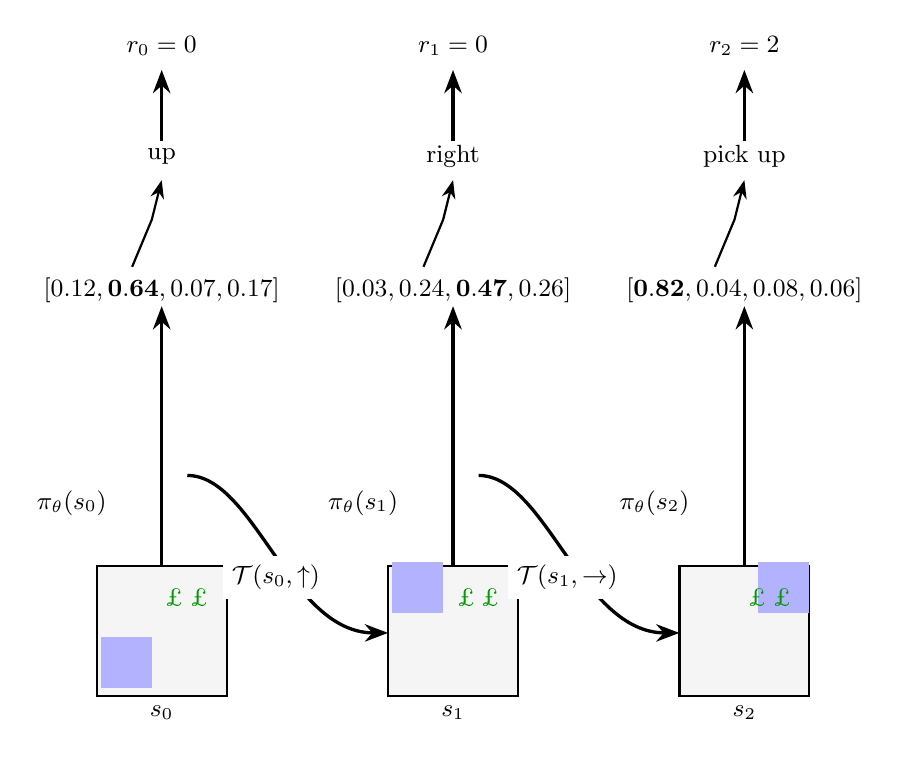
\begin{tikzpicture}[>=Stealth,font=\small]
  \state{0}{0}{$[0.12,\mathbf{0.64},0.07,0.17]$}{up}{$r_0=0$}{.05}{.05}
  \state{3.7}{1}{$[0.03,0.24,\mathbf{0.47},0.26]$}{right}{$r_1=0$}{1}{.05}
  \state{7.4}{2}{$[\mathbf{0.82},0.04,0.08,0.06]$}{pick up}{$r_2=2$}{1}{1}
  \draw[->,very thick] (1.15,-1.1) .. controls (2,-1.1) and (2.45,-3.1) .. (3.7,-3.1)
    node[midway,below,fill=white] {$\mathcal T(s_0,\uparrow)$};
  \draw[->,very thick] (4.85,-1.1) .. controls (5.7,-1.1) and (6.15,-3.1) .. (7.4,-3.1)
    node[midway,below,fill=white] {$\mathcal T(s_1,\rightarrow)$};
\end{tikzpicture}
\end{document}
